\chapter{Experimentación y evaluación del desempeño de la red}
\chaptermark{Experimentación y evaluación}

\noindent
\lettrine[lines=2, lhang=0.33, loversize=0.25]{\textbf{E}}{n}\
este capítulo se detallarán los experimentos hechos con la arquitectura expuesta\
anteriormente. La metodología llevada a cabo consistió en reunir la mayor cantidad\
posible de datos para seguir con los procedimientos descritos en la Sección \ref{sec:arq-accion}.\
Los alcances de los experimentos serán descritos más adelante, dejando en claro\
las restricciones de tiempo (para la realización de la tesis) y capacidad de equipo\
de cómputo disponible.\par
Con respecto a lo último mencionado, para los cómputos de mayor desempeño se utilizó una\
\textbf{tarjeta gráfica} (\emph{GPU}, por sus siglas en inglés) \emph{GeForce GTX 1080 Ti}\
de la marca \emph{NVIDIA}\footnote{
  Para mayor información con respecto al modelo \emph{GeForce GTX 1080 Ti},\
  consultar el sitio \url{http://la.nvidia.com/graphics-cards/geforce/pascal/la/gtx-1080-ti}.
}. Es común que en aprendizaje profundo se usen este tipo de componentes, que originalmente\
se construyen para el mundo de los videojuegos.

\section{Estructura del conjunto de datos} \label{sec:dataset}

\noindent
Como ya fue mencionado anteriormente, los datos se obtuvieron del sitio \verb+MemeGenerator.net+%
\footnote{\url{https://memegenerator.net}}.\
La información recabada en este sitio es reunida a través de usuarios alrededor del mundo,\
quienes de manera libre tienen la posibilidad de generar un nuevo meme. El sitio, además,\
agrupa a los memes en personajes (Figura \ref{meme-characters}) y los jerarquiza en base a\
su popularidad%
\footnote{
  Más aún, cualquier usuario puede crear libremente un personaje nuevo, lo que habilita la idea de\
  buscar y agrupar los memes de acuerdo a su personaje.
}.\par
En total se reunieron \textbf{4379} personajes del sitio web antes mencionado. Por cada uno de ellos\
el número de leyendas usadas para entrenar varía según los resultados obtenidos en cada experimento.\
Considerando que es necesario dividir un conjunto de datos en subconjuntos de entrenamiento y\
validación%
\footnote{
  Usualmente esta división se realiza muestreando aleatoriamente del $70$ al $80\%$ de los datos\
  para entrenamiento y del $30$ al $20\%$ para validación.
}, podemos afirmar que el tamaño de los datos de entrenamiento es pequeño en relación a otros\
conjuntos como \emph{ImageNet}.

\begin{figure}[h]
  \centering
  \begin{minipage}[l]{0.3\linewidth}
    
\includegraphics[width=\linewidth]{meme1}
  \end{minipage}\hfill
  \begin{minipage}[r]{0.3\linewidth}
    
\includegraphics[width=\linewidth]{meme2}
  \end{minipage}\hfill
  \begin{minipage}[r]{0.3\linewidth}
    
\includegraphics[width=\linewidth]{meme3}
  \end{minipage}
  \begin{minipage}[r]{0.3\linewidth}
    
\includegraphics[width=\linewidth]{meme4}
  \end{minipage}\hfill
  \begin{minipage}[r]{0.3\linewidth}
    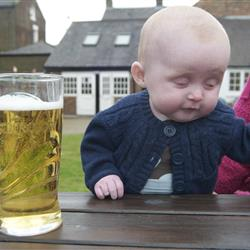
\includegraphics[width=\linewidth]{meme5}
  \end{minipage}\hfill
  \begin{minipage}[r]{0.3\linewidth}
    
\includegraphics[width=\linewidth]{meme6}
  \end{minipage}
  \begin{minipage}[r]{0.3\linewidth}
    
\includegraphics[width=\linewidth]{meme7}
  \end{minipage}\hfill
  \begin{minipage}[r]{0.3\linewidth}
    
\includegraphics[width=\linewidth]{meme8}
  \end{minipage}\hfill
  \begin{minipage}[r]{0.3\linewidth}
    
\includegraphics[width=\linewidth]{meme9}
  \end{minipage}
  \caption{
    Ejemplos de personajes populares del sitio \url{https://memegenerator.net}.
    La mayoría de ellos gozaba de gran popularidad entre los años 2009 y 2013;
    la evolución de la viralidad de los mismos y el surgimiento de otros sitios web
    para compartir memes son algunas causas que pueden explicar su ``extinción''.
    (Tomado de \url{https://memegenerator.net}.)
  }
  \label{meme-characters}
\end{figure}

Mediante una búsqueda \emph{por profundidad}, a través del árbol de páginas web, definido por cada uno de los personajes\
del sitio, uno encuentra una gran cantidad de leyendas separadas de la imagen de su personaje asociado.\
Es decir, por cada personaje se extrae una imagen y tantas leyendas como sea posible (Figura \ref{meme-separation}).\par
Para llevar a cabo este fin, se programó un \textbf{rastreador web} (\emph{web crawler}) para llevar a cabo\
la búsqueda de la información y la acumulación de los datos. Se escribió un programa en el lenguaje de\
programación \textbf{Python} (versión 3.6)\footnote{\url{https://www.python.org}} con la biblioteca\
\textit{Scrapy} (versión 1.4.0)\footnote{\url{https://scrapy.org}}, la cual organiza hilos de ejecución concurrentes\
para obtener el contenido de las \verb+URL+'s necesarias mediante peticiones \verb+GET+ de \verb+HTTP+.\
Al final, se organizaron los datos bajo la jerarquía presente en la Figura \ref{file-hierarchy}.

\begin{figure}[h]
  \centering
  \begin{minipage}[l]{\linewidth}
    \dirtree{%
      .1 personaje-1/.
      .2 personaje-1{.}csv.
      .2 personaje-1{.}jpg.
      .2 personaje-1-metadata{.}csv.
      .1 personaje-2/.
      .2 personaje-2{.}csv.
      .2 personaje-2{.}jpg.
      .2 personaje-2-metadata{.}csv.
      .1 {.}.
      .1 {.}.
      .1 {.}.
      .1 personaje-n/.
      .2 personaje-n{.}csv.
      .2 personaje-n{.}jpg.
      .2 personaje-n-metadata{.}csv.
    }
  \end{minipage}
  \caption{
    Como se observa, los datos se guardaron bajo el formato \texttt{CSV}, asociando cada leyenda con la \texttt{URL}
    de su meme asociado y su idioma de origen (Figura \ref{meme-file}). Se estima que un $90\%$ de datos está en inglés.
  }
  \label{file-hierarchy}
\end{figure}

\begin{figure}[H]
  \centering
  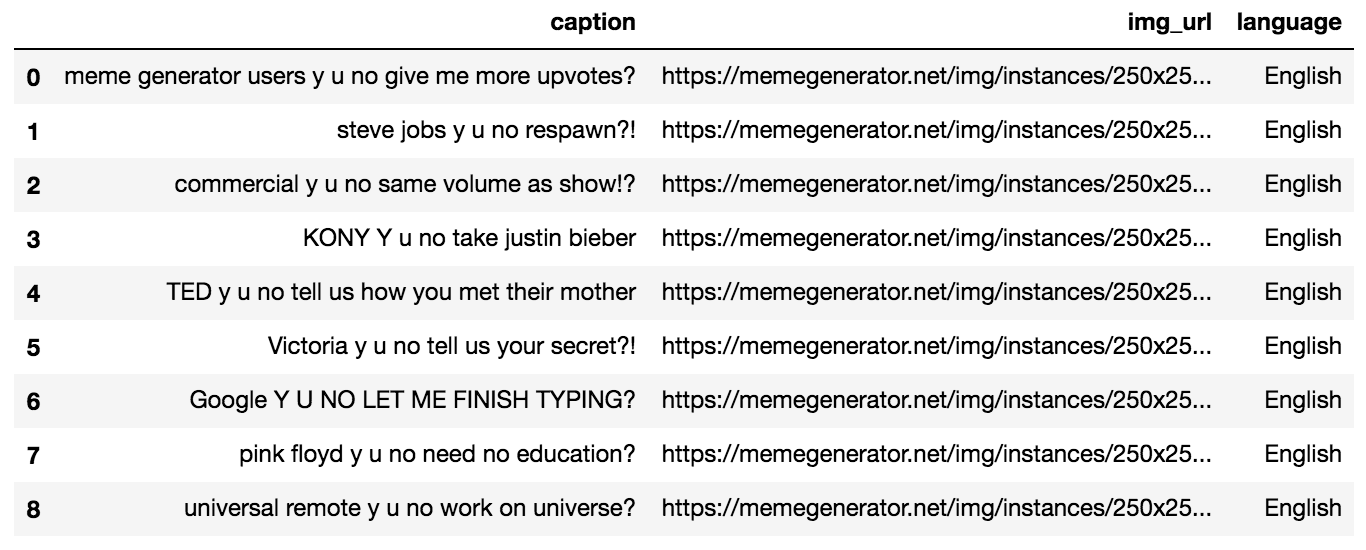
\includegraphics[width=\textwidth]{meme-file}
  \caption{
    De esta manera se guardaron cada una de las leyendas de cada personaje.
  }
  \label{meme-file}
\end{figure}

\begin{figure}
  \centering
  \begin{minipage}[l]{\linewidth}
    
\includegraphics[width=\linewidth]{thesis-i-demand-trial-by-combat}
  \end{minipage}\hfill
  \begin{minipage}[r]{0.5\linewidth}
    
\includegraphics[width=\linewidth]{tyrionlannister}
  \end{minipage}\hfill
  \begin{minipage}[r]{0.5\linewidth}
    \verb+thesis  i demand trial by combat+
  \end{minipage}
  \caption{
    La ilustración de la parte superior constituye a un meme que integra a un personaje con su leyenda y
    es el objeto que se propaga a través de Internet. Los datos que se reunieron se separaron como se
    indica en la ilustración de la parte inferior.
    (Tomado de \url{https://memegenerator.net}.)
  }
  \label{meme-separation}
\end{figure}

\section{Generación de leyendas}

\noindent
El modo \verb+inferencia+ del modelo consiste en generar una leyenda para una imagen de entrada.\
Dada la manera con la cual se representa el modelo de lenguaje aprendido del conjunto de datos\
de entrenamiento, sabemos que por cada palabra hay una distribución de probabilidad que evalúa\
qué tan viable es que cada palabra del vocabulario sea la que sigue. Por lo tanto, muchas veces\
conviene observar los $k$ enunciados que \emph{mejor} describen una imagen, maximizando la\
probabilidad conjunta entre cada una de las palabras que los componen (en orden).\par
La \textbf{búsqueda por haces} (\emph{beam search}, en inglés) es un algoritmo que logra calcular\
enunciados de \emph{``máxima verosimimilitud''}. El procedimiento incorpora a un agente cuyo\
objetivo es encontrar el camino de mayor \emph{peso} posible en una máquina de estados, en la cual solo\
tiene conocimiento del estado actual y los pesos para llegar a los vecinos del mismo. La salida\
del algoritmo muestra los $k$ enunciados más viables para cierta imagen. El agente, entonces\
registra de manera paralela las $k$ palabras de mayor probabilidad que sucedan a la palabra anterior.\par
Normalmente, esto se programa mediante $k$ hilos de ejecución en paralelo. Cada uno se inicializa\
aleatoriamente con las $k$ palabras de inicio de mayor probabilidad. En el paso $t$, cada\
hilo vuelve a calcular los $k$ siguientes mejores estados (un total de $k^2$ estados) y, al final,\
el agente se queda con los mejores $k$ para proceder al paso $t+1$. En este caso, se consideraron\
los $k=3$ mejores enunciados para cada imagen.

\section{Experimentos}

\noindent
Los experimentos realizados obedecen a lo sugerido por la teoría presentada en los dos capítulos anteriores.\
Se buscó seguir la metodología sugerida por el \emph{estado del arte} (\cite{DBLP:journals/corr/VinyalsTBE16}).\
Por ello, se eligió trabajar con el lenguaje de programación Python (versión 3.6) y las bibliotecas\
\textbf{Tensorflow} (versión 1.3.0)\footnote{\url{https://www.tensorflow.org}} y \textbf{Keras}\
(versión 2.0.9)\footnote{\url{https://keras.io}}.\par
Ambas bibliotecas son obra \emph{reciente} de la división de código abierto de \emph{Google}.\
\emph{Tensorflow} surgió como una iniciativa para compartir la manera en que dicha empresa despliega\
sus proyectos que involucran aprendizaje profundo. El paradigma que se sigue consiste en definir un\
grafo dirigido de \emph{tensores} como nodos, en el cual fluirá la información\footnote{
  En cada nodo del grafo, se definen \emph{operaciones} (lectura y escritura de archivos, operaciones\
  matriciales, etc.) y se da la posibilidad de especificar si van a correr en un GPU, si se cuenta con uno.
}; acto seguido, se ``compila'' el modelo y se levanta una sesión para ejecutarlo. Así, \emph{Tensorflow}\
utiliza la sintaxis de \emph{Python} para construir redes neuronales en un mayor nivel.\par
Por otro lado, \emph{Keras} se define a sí misma como una interfaz de programación de aplicaciones (\emph{API})\
de alto nivel, que utiliza como motor de ejecución a \emph{Tensorflow}. Es decir, el programador es capaz\
de escribir código que defina una red neuronal y se ejecute secuencialmente. \emph{Keras}, además,\
facilita la tarea de definir un modelo profundo con una sintaxis más amigable que la de \emph{Tensorflow}\
y configura algunos \emph{hiper-parámetros} de ésta, con el fin de facilitar el prototipado de redes neuronales\
profundas.

\subsection{Experimentos exploratorios}

\noindent
Vinyals, \emph{et al} presentan tanto en \cite{DBLP:journals/corr/VinyalsTBE14} como en \cite{DBLP:journals/corr/VinyalsTBE16}\
el \emph{estado del arte} de los modelos neuronales capaces de generar descripciones a partir de imágenes.\
Por ende, el primer paso experimental consistió en replicar el entrenamiento completo, usando el conjunto de datos\
\emph{ImageNet}.\par
Utilizando pesos pre-entrenados%
\footnote{
  \emph{Tensorflow} provee un conjunto de modelos previamente entrenados bajo un subconjunto de\
  \emph{ImageNet} (\url{http://www.image-net.org/challenges/LSVRC/2012/}). Esto ahorra tiempo en la vectorización\
  de imágenes. Para mayor información, consultar el sitio\
  \url{https://github.com/tensorflow/models/tree/master/research/slim\#tensorflow-slim-image-classification-library}.
} de Inception V3, se realizó el proceso de generar un tensor de incrustaciones de las imágenes de ImageNet\
en un espacio vectorial. Acto seguido se alimentó una LSTM con dicho tensor, como memoria inicial, y se\
entrenó utilizando las leyendas asociadas a cada imagen.\par
Dentro de las ventajas consecuentes de este experimento, está el tener una implementación\
de una LSTM para ser entrenada de nuevo, con cualquier memoria inicial. El desempeño del entrenamiento\
se ilustra en la Figura \ref{exp1}. Es importante destacar que, dadas las altas dimensiones con las que\
se trabaja en cada capa, se estima que se requieren alrededor de 1 millón de épocas para que el error\
dado por la entropía cruzada se estabilice en un valor mínimo (este comportamiento es común para la mayoría\
de los experimentos subsecuentes).\par
El objetivo principal de este primer experimento era familiarizarse con el uso de las implementaciones y la\
tecnología necesaria para realizar aprendizaje profundo. Por ende, se decidió dejar a un lado la evaluación\
del desempeño de este modelo neuronal, mediante un conjunto de datos independiente del de entrenamiento y\
validación.

\begin{figure}[H]
  \centering
  \begin{minipage}[c]{\linewidth}
    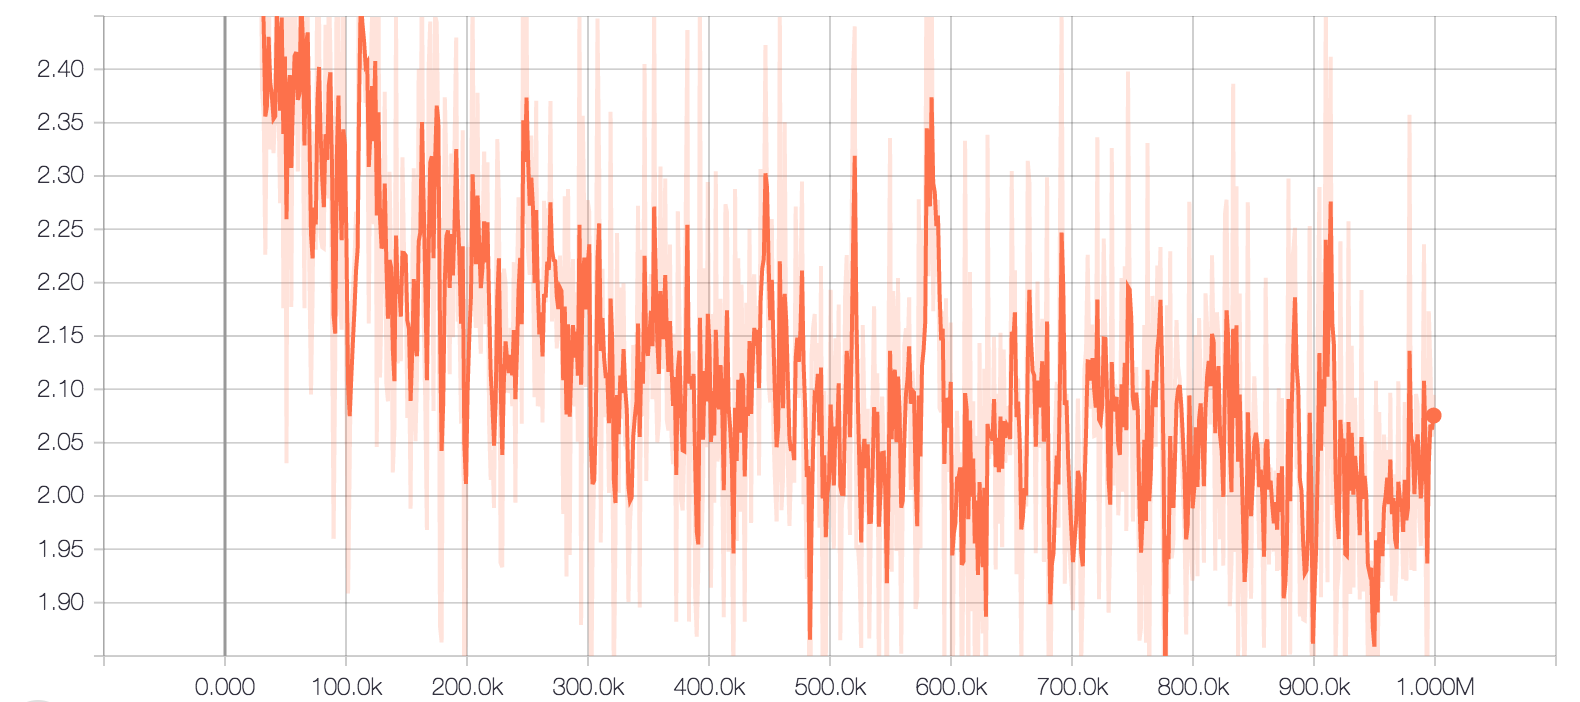
\includegraphics[width=\linewidth]{exp1-1}
  \end{minipage}\hfill
  \begin{minipage}[c]{\linewidth}
    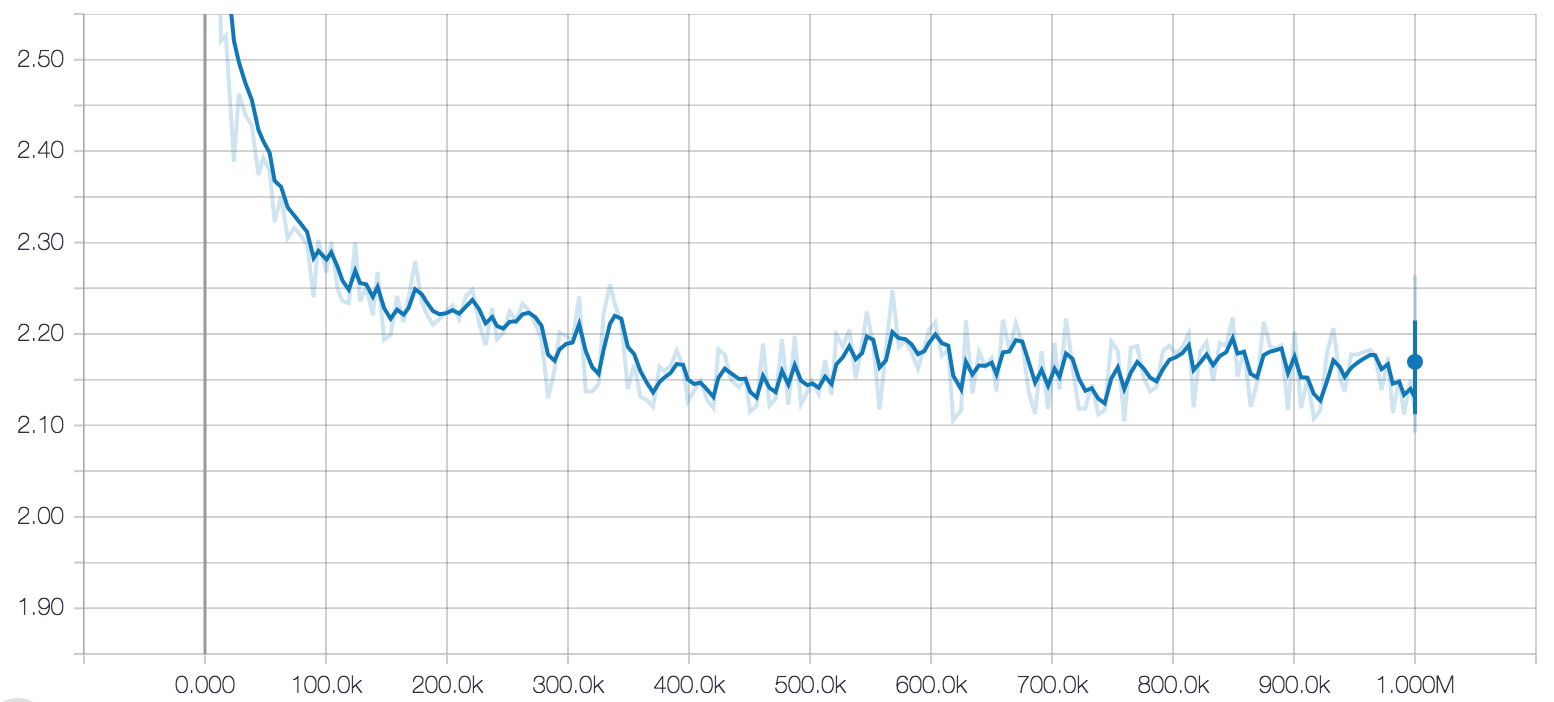
\includegraphics[width=\linewidth]{exp1-2}
  \end{minipage}
  \caption{
    Función de error de entropía cruzada para el primer experimento exploratorio.
    En el gráfico de la parte superior se muestra el error
    a través de cada época del entrenamiento, mientras que el de la parte inferior se
    calculó por medio de un conjunto de datos de \emph{validación} (de menor tamaño que el de entrenamiento).
    Ambos gráficos indican el valor de la entropía cruzada (eje de las ordenadas) a través del
    tiempo (eje de las abscisa).
    (Fuente: elaboración propia.)
  }
  \label{exp1}
\end{figure}

Tenemos, ahora, una CNN que es ``experta'' en etiquetar imágenes con detalles muy generales. Vale la pena,\
entonces, probarla con el conjunto de datos de memes. Buscamos ver, de entrada, que sea capaz de distinguir\
entre dos imágenes distintas (mediante representaciones vectoriales muy diferentes), que además se\
refleje en la discrepancia entre las leyendas generadas. Para ello, diseñamos un experimento en el\
que entrenamos una LSTM con una memoria inicial dada por los códigos convolucionales obtenidos\
a partir de \textbf{97} personajes del conjunto de datos. Estos personajes pasarán por la red\
\emph{Inception V3} pre-entrenada del experimento anterior.

\begin{figure}[h]
  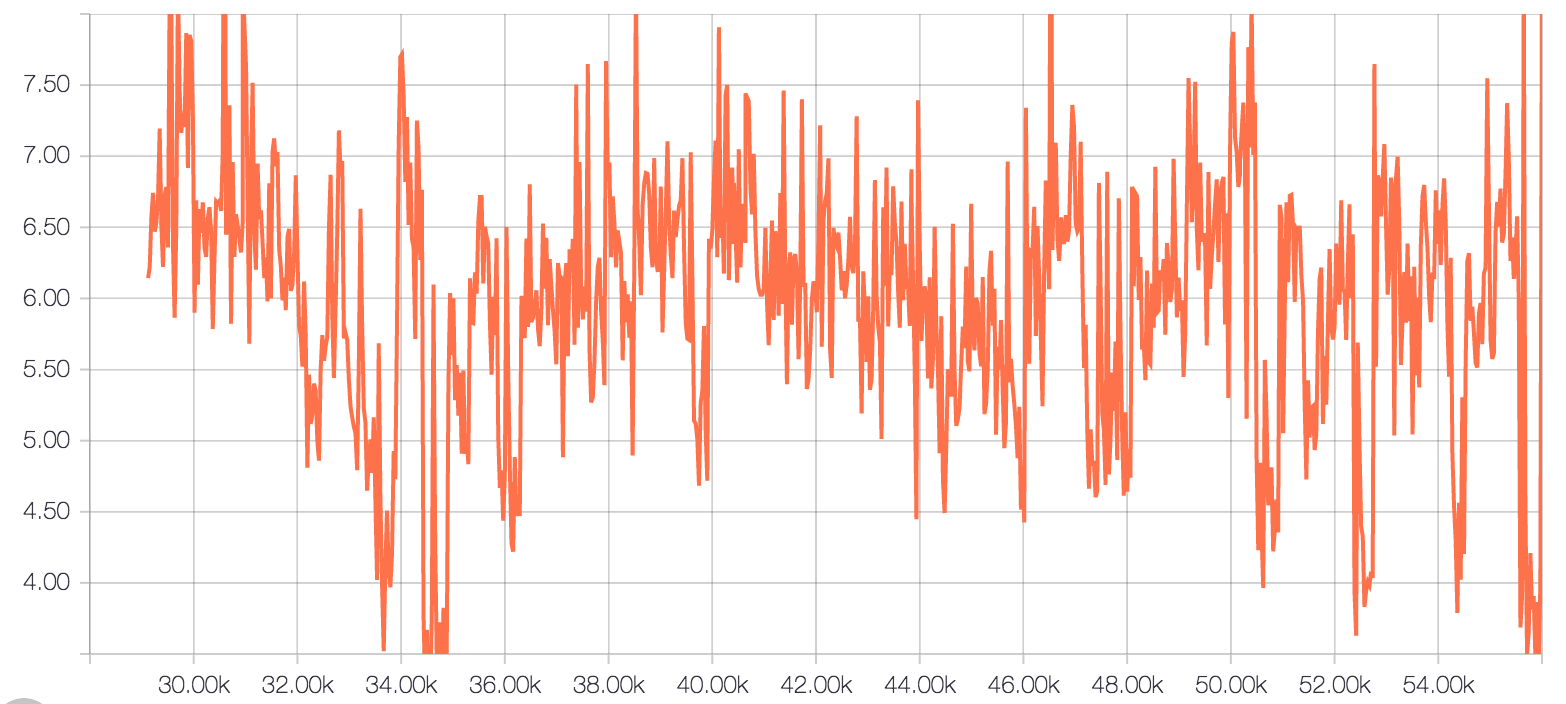
\includegraphics[width=\linewidth]{exp4-1}
  \caption{
    Función de error para el experimento que utiliza la CNN \emph{Inception V3}
    con pesos pre-entrenados, sin ser afinada.
    (Fuente: elaboración propia.)
  }
  \label{exp4}
\end{figure}

Cada personaje posee un promedio de 700 leyendas, pues el número total de leyendas por personaje varía\
según la popularidad del mismo. Cabe destacar que el vocabulario construído tuvo alrededor de 20 mil palabras distintas.\
El desempeño fue deficiente tanto en entrenamiento (Figura \ref{exp4}) como en resultados \emph{anecdóticos}.\
Las siguientes observaciones fueron notables:
\begin{itemize}
\item los códigos convolucionales resultantes del paso por la CNN fueron indistinguibles entre\
  una imagen y otra, dejando en claro la necesidad de realizar una afinación);
\item lo anterior provocó que las leyendas fueran todas iguales para imágenes distintas;
\item el elevado tamaño del vocabulario no favoreció al modelo para poder asignar probabilidades,\
  condicionales, al momento de generar frases (repetición palabras de manera contigua).
\end{itemize}\par
El bajo desempeño de este experimento motivó a \emph{no} realizar una evaluación de los resultados pero\
trajo consigo dos hipótesis para considerarse. La primera de ellas consiste en afinar la red \emph{Inception V3}\
con el conjunto de datos de memes, pues se cree que el modelo implícito en sus parámetros pre-entrenados\
explora detalles mucho más generales de los requeridos para clasificar imágenes como las mostradas en la\
Figura \ref{meme-characters}. Dado el tamaño del conjunto de datos, se plantea, de igual manera, como\
hipótesis, la viabilidad de que una CNN más \textbf{superficial} (menos profunda) tenga éxito al\
generar códigos convolucionales.

\subsection{Experimentos que involucran la afinación de una arquitectura convolucional profunda}

\noindent
Para aprovechar la especialización que posee \emph{Inception V3}, de reconocer patrones simples en\
imágenes, afinamos dicho modelo con un clasificador de memes. Dado que el conjunto de datos\
presentado en la Sección \ref{sec:dataset} no está dividido en ``categorías'' de memes, resulta difícil\
realizar una tarea de aprendizaje supervisado con una CNN.\par
Por otro lado, dadas las características de las imágenes de los memes, existe un patrón más o menos definido\
(rostro del personaje centrado en la imagen) que puede ser explotado contra la tarea general de aprender\
a clasificar \emph{ImageNet}. Esto nos brindó la solución para poder afinar a \emph{Inception V3}: colocar\
una capa MLP, al final de la red, con salida de dos dimensiones para decidir si la entrada es, o no es,\
un meme.\par
Las imágenes \emph{``no memes''} utilizadas en este punto se tomaron aleatoriamente muestreando 4379 de \emph{ImageNet}.\
Se trabajó bajo la premisa de que la profundidad de la red\
alcanzará para generalizar la identificación de las características presentes en un meme. Después de todo,\
nuestro conjunto de datos posee imágenes de mucho menor complejidad que las existentes en \emph{Inception V3}.
En total, se dejaron 3065 imágenes (memes y no memes) para entrenamiento, 657 para validación y 657 para evaluación;
el resultado de este proceso se ilustra en la Figura \ref{exp2}. El desempeño fue bastante favorable,\
ya que se minimizó considerablemente el error de la entropía cruzada. Además, con el conjunto de\
evaluación se corroboró dicho rendimiento mediante los gráficos de las métricas de \emph{precisión}%
\footnote{
  La \textbf{precisión} (\emph{accuracy}, en inglés) puede ser entendida como el porcentaje\
  de aciertos que tiene el modelo al intentar predecir un lote de datos. Se busca, entonces,\
  que su valor esté muy cercano a 1.
} y \emph{error medio absoluto}%
\footnote{
  El \textbf{error medio absoluto} es la diferencia promedio que existe entre los valores\
  estimados por un modelo ($\hat{Y}$) y los valores reales de un conjunto de datos ($Y$). Esto\
  se calcula con la expresión
  \[\frac{\sum_{i=1}^n \hat{Y}_i - Y_i}{n}.\]
} (Figura \ref{eval:exp2}).

\begin{figure}[h]
  \begin{minipage}[c]{\linewidth}
    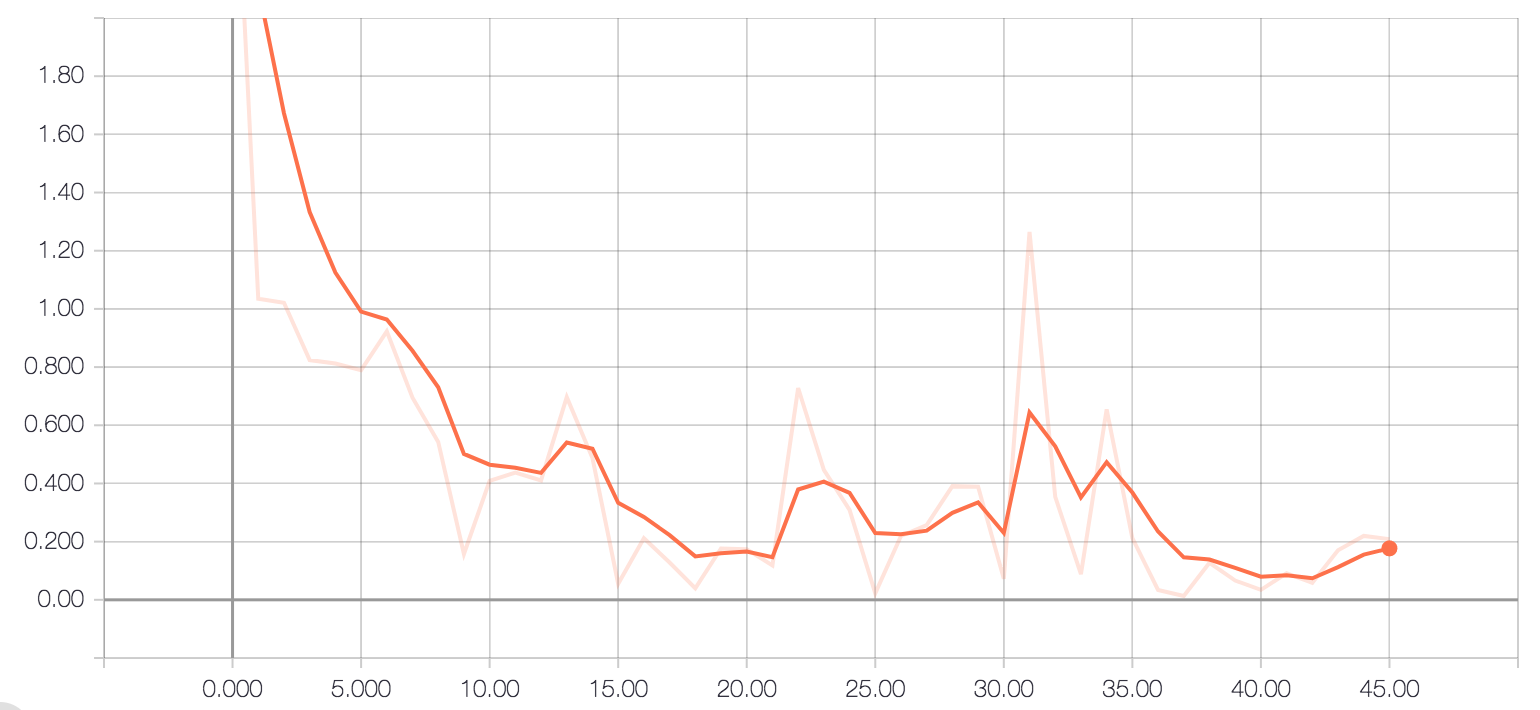
\includegraphics[width=\linewidth]{exp2-1}
  \end{minipage}\hfill
  \begin{minipage}[c]{\linewidth}
    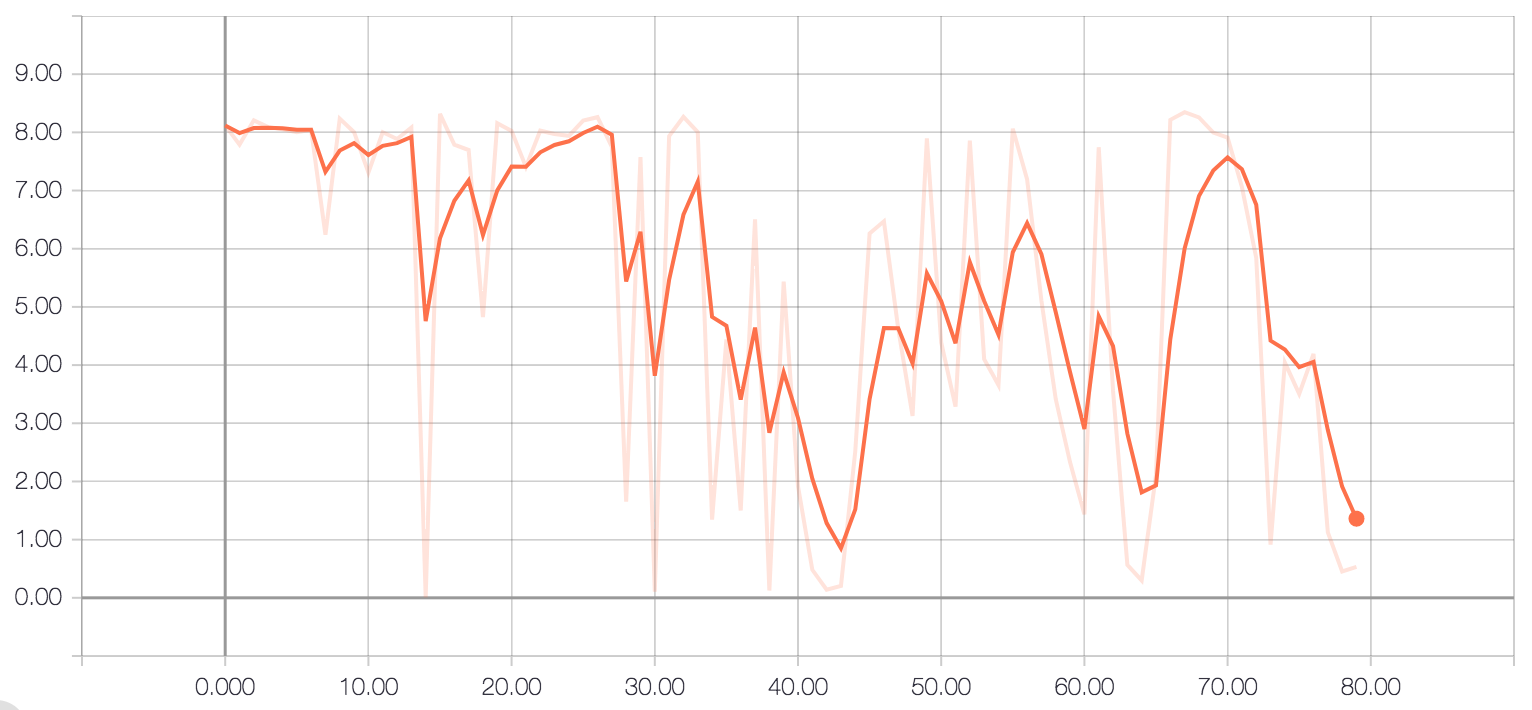
\includegraphics[width=\linewidth]{exp2-2}
  \end{minipage}
  \caption{
    Funciones de error de entrenamiento y validación (gráfico de arriba y de abajo,
    respectivamente) para la afinación de \emph{Inception V3}.
    Esto es, entrenar un clasificador entre lo que es un meme y lo que no es. Se quita\
    la última capa y se añade un MLP con dos dimensiones de salida.
    (Fuente: elaboración propia.)
  }
  \label{exp2}
\end{figure}

\begin{figure}[H]
  \centering
  \begin{minipage}[c]{\linewidth}
    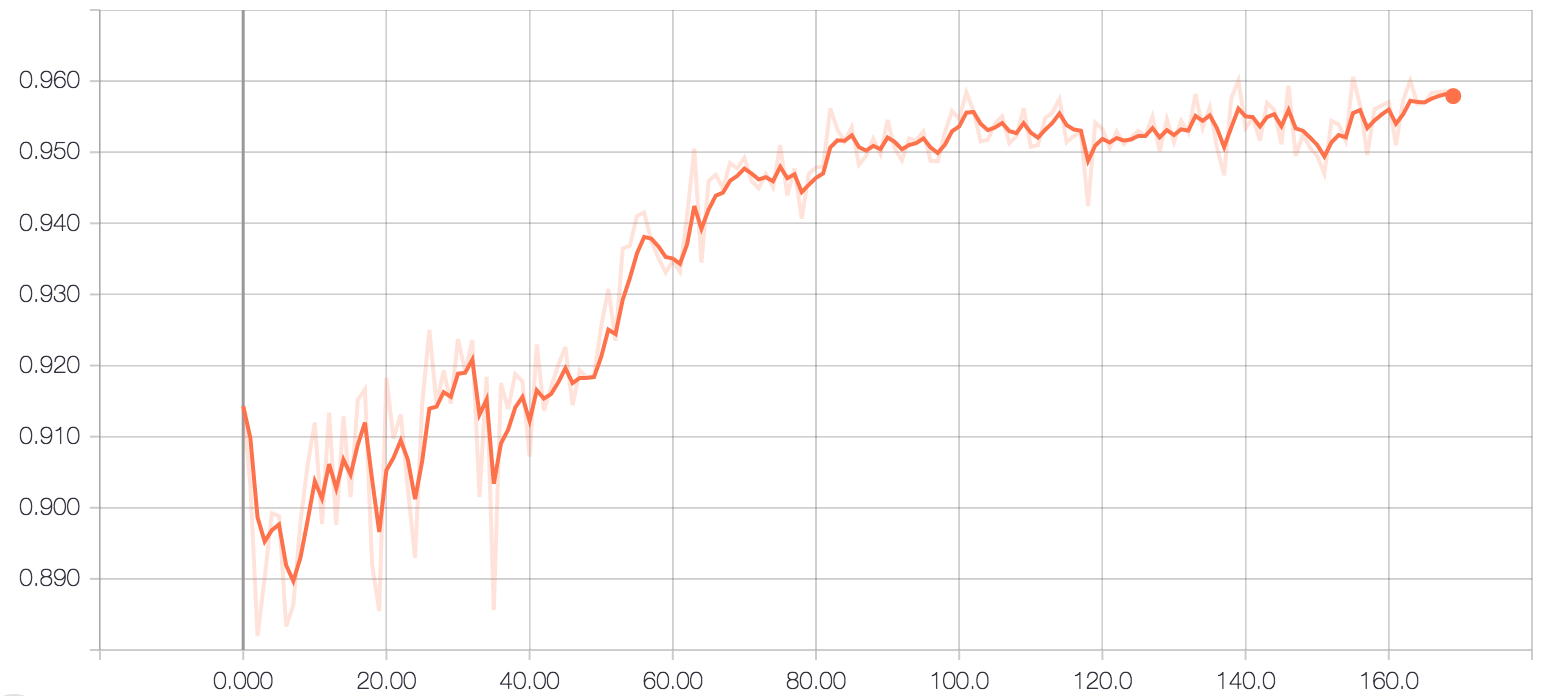
\includegraphics[width=\linewidth]{exp2-3}
  \end{minipage}\hfill
  \begin{minipage}[c]{\linewidth}
    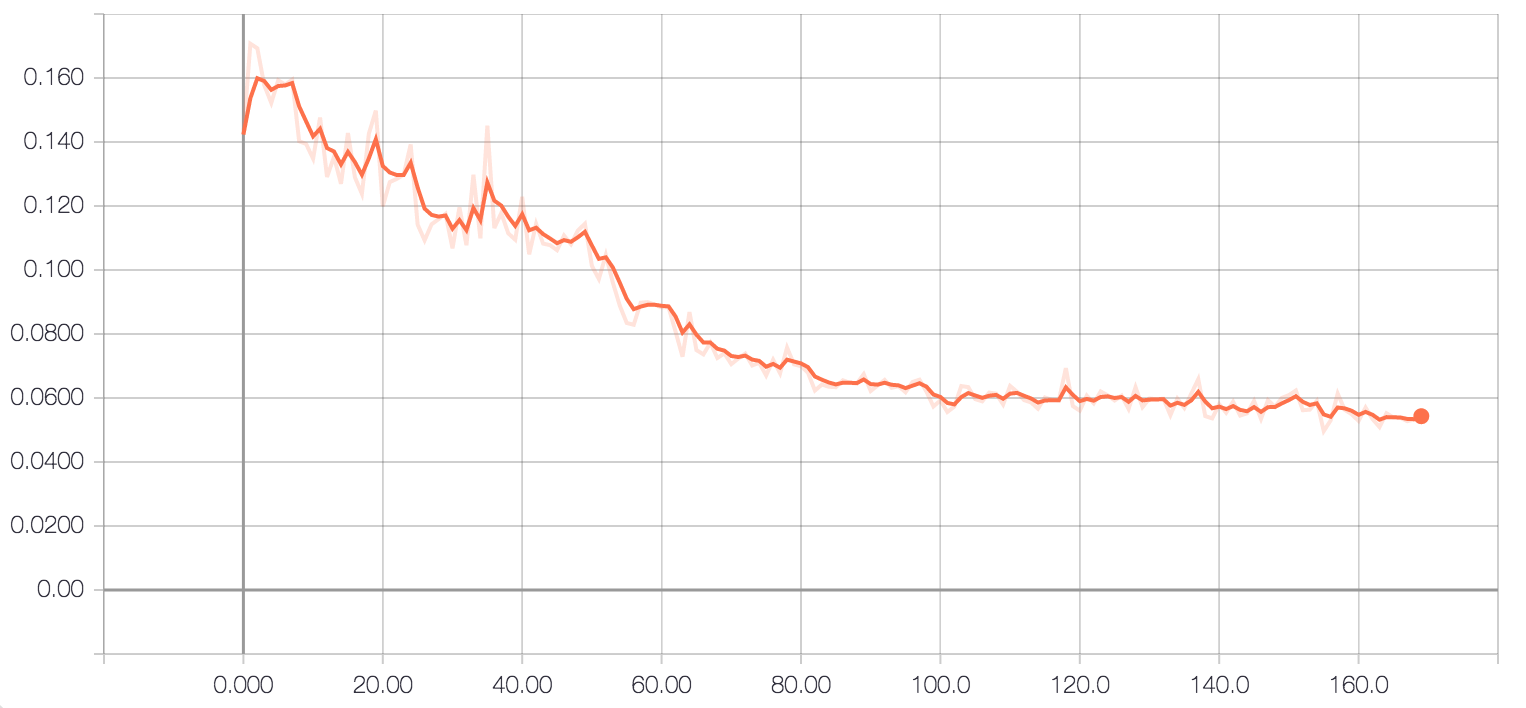
\includegraphics[width=\linewidth]{exp2-4}
  \end{minipage}
  \caption{
    Dos funciones de evaluación para la afinación de \emph{Inception V3}.
    El gráfico de la parte superior muestra la \emph{precisión} con la que el modelo realiza
    sus clasificaciones, mientras que el gráfico de la parte inferior muestra el
    \emph{error medio absoluto} entre las clasificaciones hechas por el modelo contra las verdaderas.
    Ambos gráficos se generaron a partir de un muestreo del $10\%$ de los datos disponibles.
    (Fuente: elaboración propia.)
  }
  \label{eval:exp2}
\end{figure}

Una vez teniendo afinada una red neuronal profunda, surge la inquietud de ver si esto ayuda\
a mejorar el primer experimento en el que se entrenó la LSTM usando memes. Por ello\
se usaron los mismos datos que los que se usaron para dicho experimetno pero\
con la \emph{Inception V3} previamente afinada. Esto provocó que entre cualesquiera\
dos imágenes diferentes, existieran dos códigos convolucionales con valores suficientemente\
distintos; lo que implica que las leyendas generadas serán también distintas.\par
El tensor de imágenes y leyendas de entrada $(I, S)$ se fue construyendo en orden,\
de manera que todas las leyendas de un solo personaje permanecían en posiciones contiguas.\
Dada la cantidad desmedida de leyendas, esto provocó que tras ciertas iteraciones se sobreentrenara\
el modelo sobre un mismo lote. Así, al probar el modo de \verb+inferencia+ del mismo,\
se podía observar claramente una tendencia por repetir la ``manera de hablar'' de un cierto personaje\
(Tabla \ref{exp5:anec}). Iteraciones más tarde, esto cambiaba para que el modelo comenzará a repetir la manera de\
hablar de otro personaje. Una de las evidencias del sobreajuste se ilustra en la Figura \ref{exp5}.\par
A pesar que las leyendas generadas aparentan tener sentido, el sobreajuste que se dio en varios\
momentos del entrenamiento motivó a realizar un mayor trabajo de procesamiento previo. En particular,\
se destaca la importancia de restringir el tamaño del vocabulario, así como de mezclar aleatoriamente\
los tensores de memoria inicial que alimentarán la LSTM. Esta última acción garantiza que no se repitan\
ciertas frases un número de veces elevado en cada lote de entrenamiento, por lo que se espera una\
reducción en el sobreajuste. Por lo tanto, se omitió la evaluación de este experimento, esperando\
resultados más apegados a la realidad de la distribución del conjunto de entrenamiento.

\begin{figure}[h]
  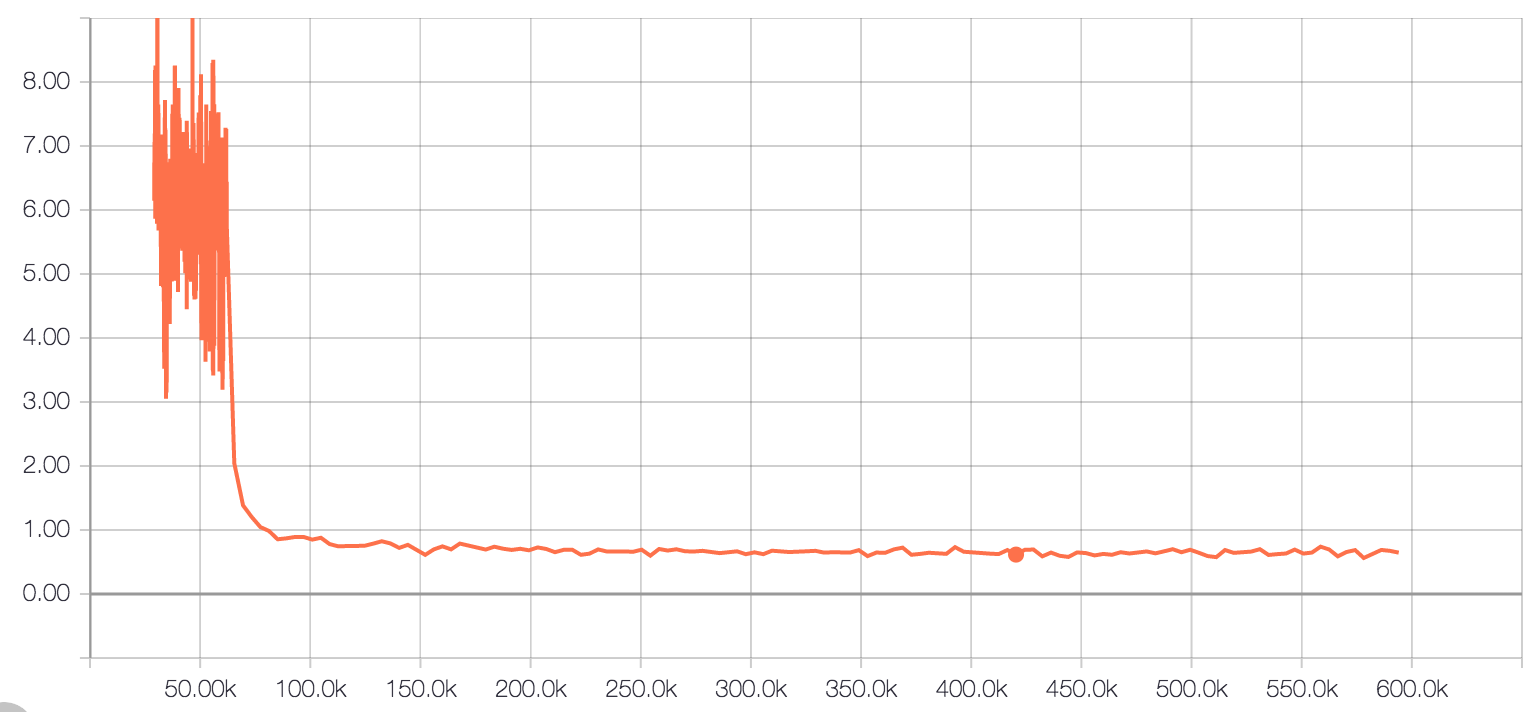
\includegraphics[width=\linewidth]{exp5-1}
  \caption{
    Función de error para el entrenamiento de la LSTM, dándole como estado inicial\
    un tensor generado a apartir de la red \emph{Inception V3} afinada.
    (Fuente: elaboración propia.)
  }
  \label{exp5}
\end{figure}

Para refinar el desempeño de la CNN afinada, el siguiente experimento se diseñó muestreando aleatoriamente\
\textbf{3416} personajes. Además, se eliminaron todas las palabras que no aparecen al menos\
5 veces en todo el conjunto de datos y se usaron únicamente 5 leyendas\
para cada personaje, con el fin de reducir el tamaño del vocabulario. Por consiguiente\
el vocabulario se redujo a 4528 palabras.\par
Previo al entrenamiento, se mezclaron los datos de manera aleatoria en el tensor $(I, S)$;\
esto provocó la diversificación en la manera con la que se generan leyendas para\
imágenes que no aparecen en el conjunto de entrenamiento. El comportamiento de la función de\
error se muestra en la Figura \ref{exp6}.

\begin{figure}[H]
  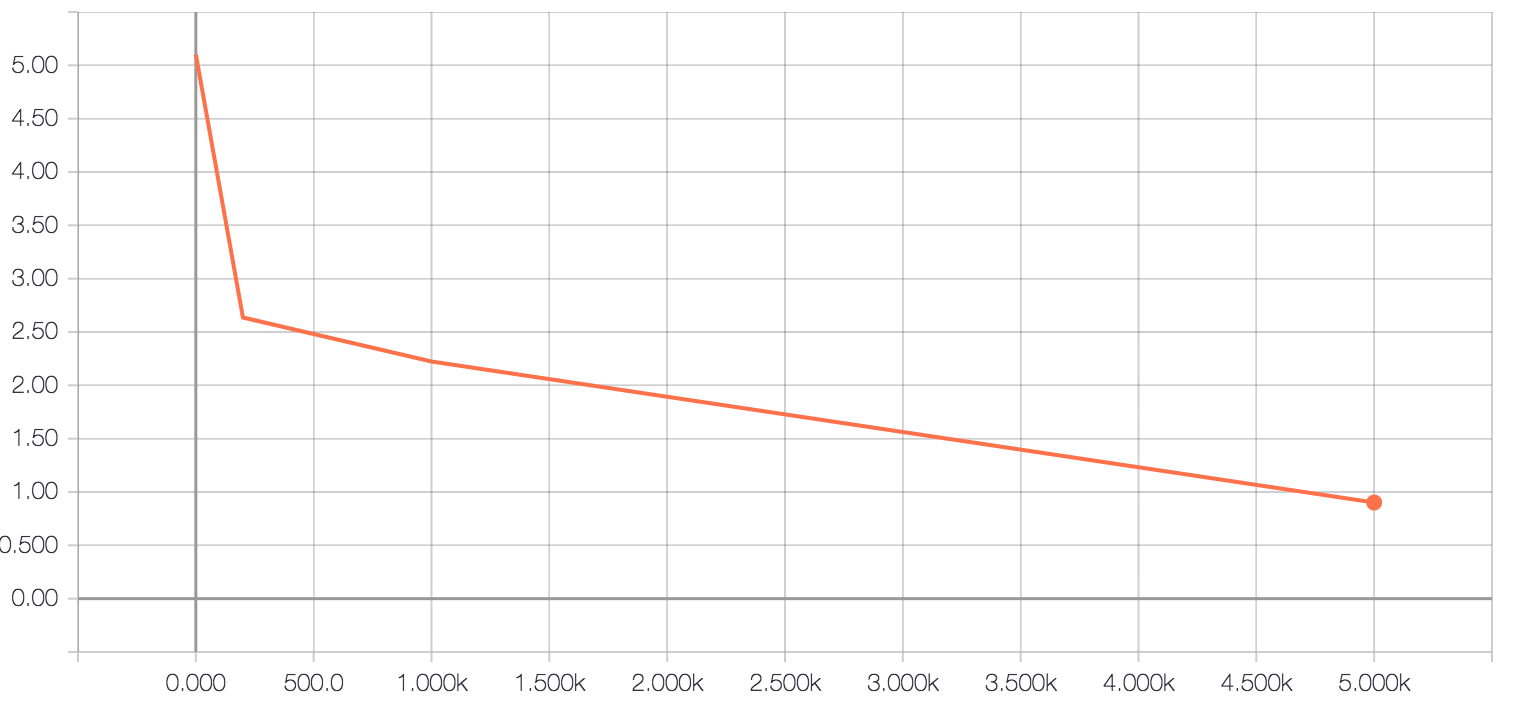
\includegraphics[width=\linewidth]{exp6-1}
  \caption{
    Función de error para el experimento que involucra la red \emph{Inception V3}
    afinada y 5 leyendas por personaje en el entrenamiento.
    (Fuente: elaboración propia.)
  }
  \label{exp6}
\end{figure}

Cualitativamente, la Figura \ref{exp6} muestra una curva descendente más suave, lo que hace pensar\
que el modelo, en efecto, aprendió a generalizar ciertos detalles del conjunto de datos. En promedio,\
podemos afirmar que el error de la entropía cruzada baja, con los cambios hechos y da cierto grado de\
confianza debido a la mezcla aleatoria de las leyendas. Por otro lado, queda la duda de qué pasaría si\
el tensor de códigos convolucionales es generado a partir de una CNN más superficial, algo que es\
válido plantearse debido al número de imágenes disponibles.\par
Este último experimento será el que mejor desempeño trae de los que usaron la red \emph{Inception V3}\
afinada. Efectuar métricas de evaluación como \emph{precisión} y \emph{error medio absoluto} es una\
práctica poco común en tareas que involucran generación de texto: la calidad de las leyendas generadas\
debe ser comparada con un modelo de lenguaje real. Por ello, en la Sección \ref{sec:metrics} presentamos\
una evaluación basada en una métrica común para el procesamiento del lenguaje natural. La Tabla\
\ref{exp6:anec} muestra algunos resultados anecdóticos de este experimento.

\subsection{Experimentos que involucran una arquitectura convolucional superficial}

\noindent
Aunque afinar una CNN profunda, previamente entrenada, es un procedimiento justificado por la literatura,\
el número máximo de imágenes que conforman el conjunto de datos sugiere otro tratamiento.\
Esto indica que entrenar una red neuronal desde cero no es una mala apuesta,\
después de todo, de acuerdo a \cite{DBLP:journals/corr/YosinskiCBL14}.\par
Ahora, presentamos el entrenamiento de una red neuronal superficial (\emph{bastante menos profunda}).\
Se usaron los mismos datos que para la afinación de \emph{Inception V3}.
La arquitectura de esta red se muestra en la Tabla \ref{capas-small},\
el desempeño del entrenamiento se ilustra en la Figura \ref{exp3}, mientras que\
la evaluación del modelo se encuentra en la Figura \ref{eval:exp3}.

\begin{table}[h]
  \resizebox{\textwidth}{!}{
    \begin{tabular}{|l|c|c|}
      \hline
      \textbf{tipo} & \textbf{tamaño de filtro} & \textbf{número de filtros}\\
      \hline \hline
      CONV & $3 \times 3$ & $32$ \\
      \hline
      CONV & $3 \times 3$ & $16$ \\
      \hline
      POOL & $2 \times 2$ & - \\
      \hline
      DROPOUT & $25\%$ de las neuronas se ignoran & - \\
      \hline
      MLP & $128$ unidades de salida & - \\
      \hline
      DROPOUT & $50\%$ de las neuronas se ignoran & - \\
      \hline
      MLP & $2$ unidades de salida & - \\
      \hline
    \end{tabular}
  }
  \caption[Nota al pie]{
    Arquitectura utilizada para entrenar una CNN superficial. Las capas
    \textbf{DROPOUT} constituyen una popular técnica de \emph{regularización}\footnotemark en
    la que se descarta un porcentaje dado de las neuronas de entrada con el fin
    de evitar un sobreajuste sobre el conjunto de datos en cuestión.
  }
  \label{capas-small}
\end{table}

\footnotetext{
  Las técnicas de \textbf{regularización}, en aprendizaje automático, añaden una
  restricción adicional al problema en cuestión para evitar que los valores
  del modelo propuesto se ajusten completamente al conjunto de datos de entrenamiento.
  Es decir, evitar el \emph{sobreajuste} y favorecer la generalización hacia datos
  no observados durante el entrenamiento.
}

\begin{figure}[H]
  \begin{minipage}[c]{\linewidth}
    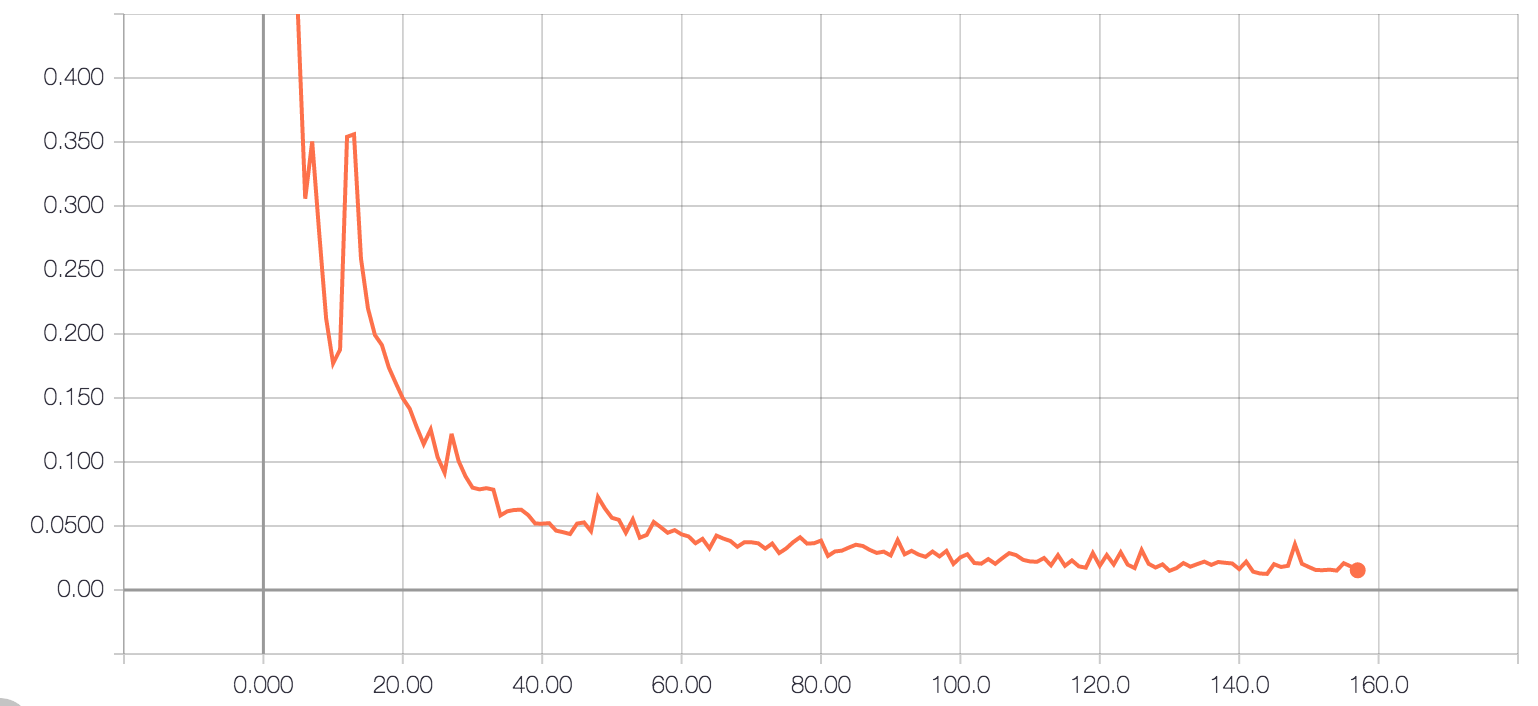
\includegraphics[width=\linewidth]{exp3-1}
  \end{minipage}\hfill
  \begin{minipage}[c]{\linewidth}
    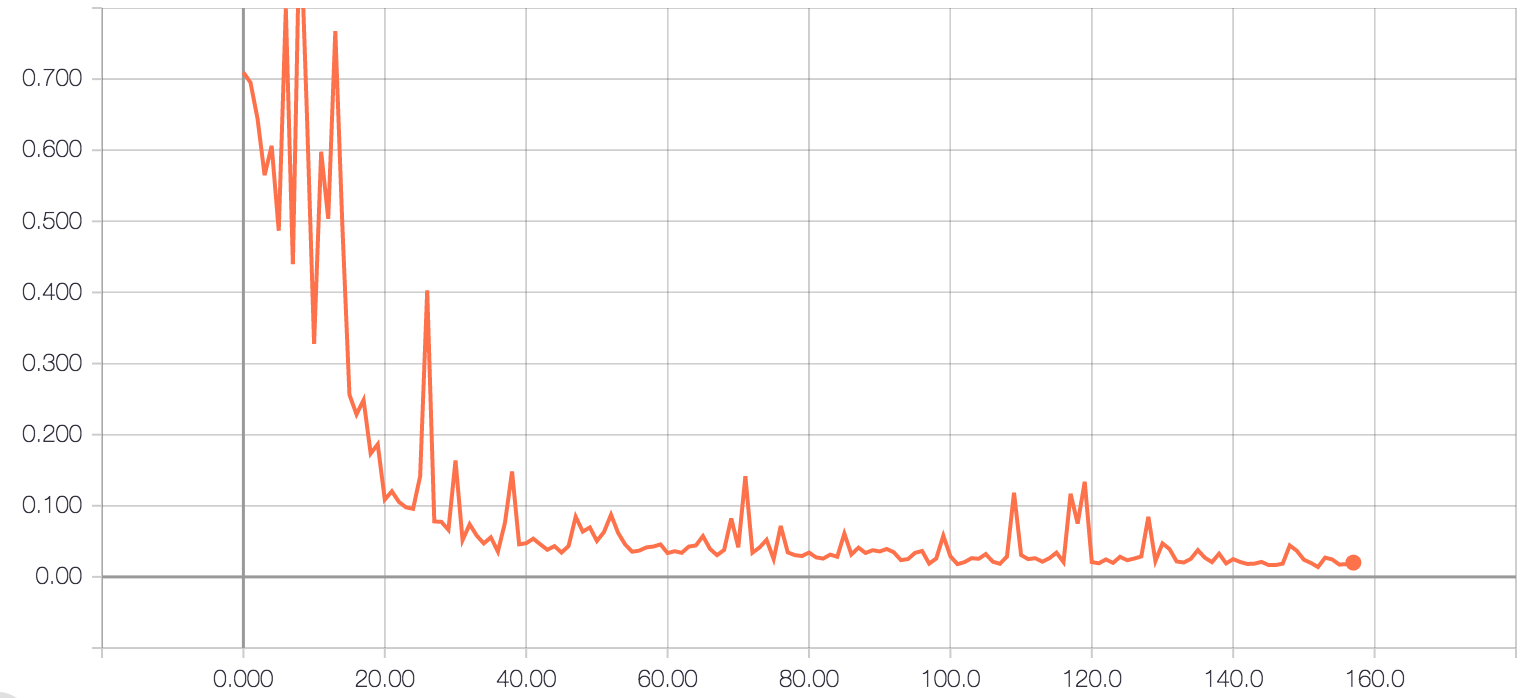
\includegraphics[width=\linewidth]{exp3-2}
  \end{minipage}
  \caption{
    Funciones de error de entrenamiento y validación (gráfico de arriba y de abajo,
    respectivamente) de la CNN superficial. Obsérvese que
    solo se requirieron alrededor de 150 épocas de entrenamiento para llegar a un
    valor óptimo; esto dado el tamaño del conjunto de datos (\emph{memes} y
    \emph{no memes}) que es bastantes órdenes de magnitud más pequeño el\
    conjunto de datos de entrenamiento presentado en la Sección \ref{sec:dataset}.
    (Fuente: elaboración propia.)
  }
  \label{exp3}
\end{figure}

Procedemos, entonces, a replicar el último experimento realizado en la sección anterior.\
Sin embargo, esta vez utilizamos la CNN superficial entrenada sobre memes y no memes.\
El entrenamiento arrojado (Figura \ref{exp7}) fue muy similar a lo observado en la\
Figura \ref{exp6}; no obstante, se logró una mejora en la calidad de las leyendas\
sin ser un detalle anecdótico muy considerable (Tabla \ref{exp7:anec}).

\begin{figure}[H]
  \centering
  \begin{minipage}[c]{\linewidth}
    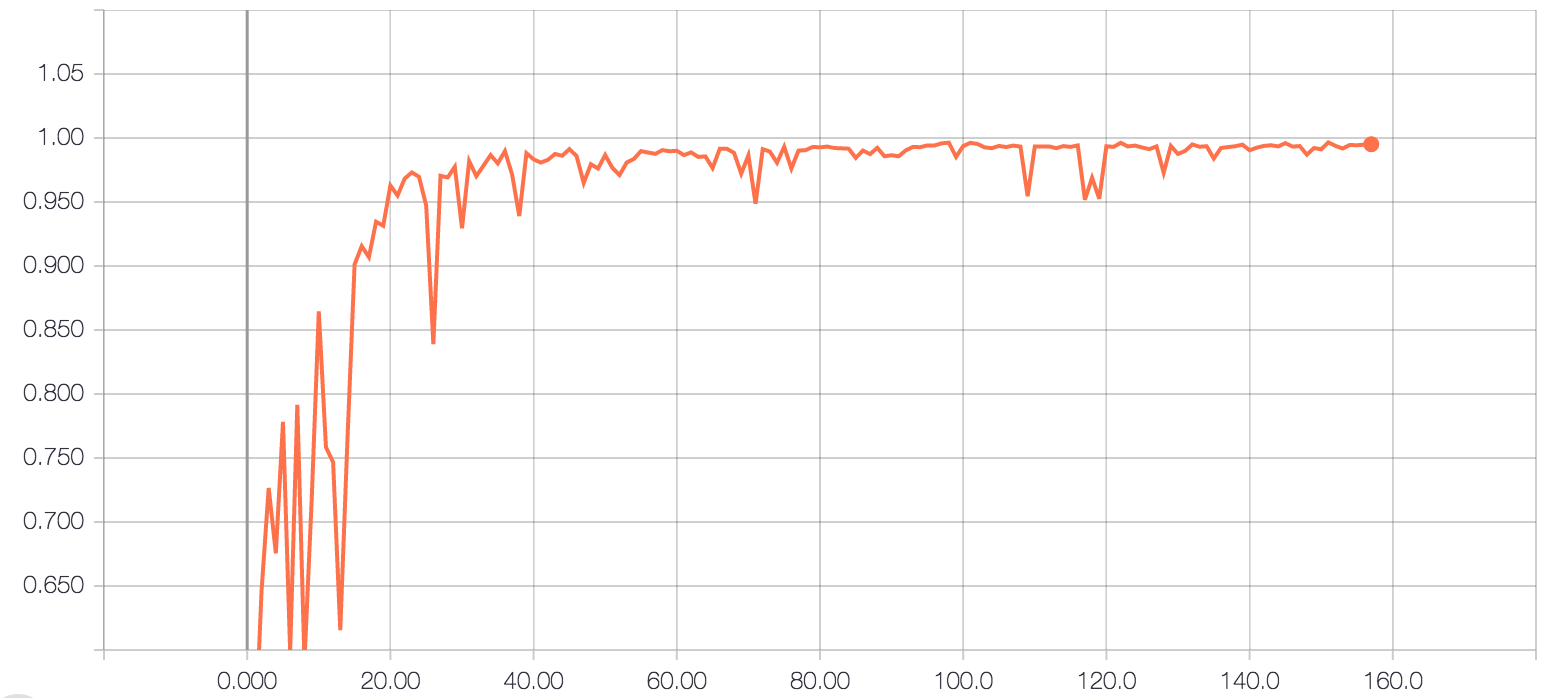
\includegraphics[width=\linewidth]{exp3-3}
  \end{minipage}\hfill
  \begin{minipage}[c]{\linewidth}
    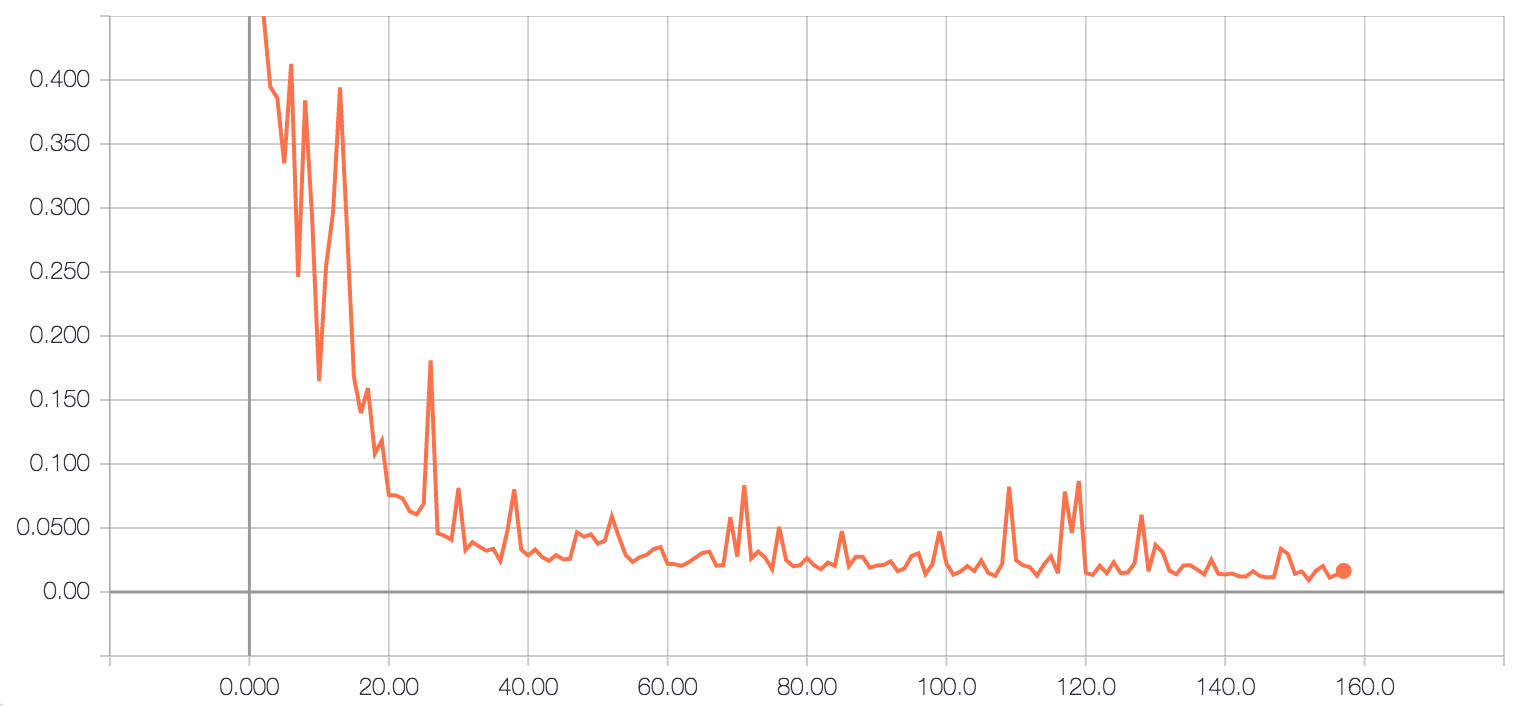
\includegraphics[width=\linewidth]{exp3-4}
  \end{minipage}
  \caption{
    Dos funciones de evaluación para el modelo convolucional superficial.
    El gráfico de la parte superior muestra la \emph{precisión} con la que el modelo realiza
    sus clasificaciones, mientras que el gráfico de la parte inferior muestra el
    \emph{error medio absoluto} entre las clasificaciones hechas modelo contra las verdaderas.
    Ambos gráficos se generaron a partir de un muestreo del $10\%$ de los datos disponibles.
    (Fuente: elaboración propia.)
  }
  \label{eval:exp3}
\end{figure}

Hasta este punto, podemos decir que hemos construido dos modelos convolucionales capaces\
de distinguir entre cualesquiera dos personajes. La tarea pendiente recae en hallar los\
(\emph{híper})-parámetros necesarios para que las leyendas generadas tengan más sentido a juicio\
de un ser humano. Por ello, reportamos un último experimento que involucra un mayor número de palabras\
por personaje.

\begin{figure}[H]
  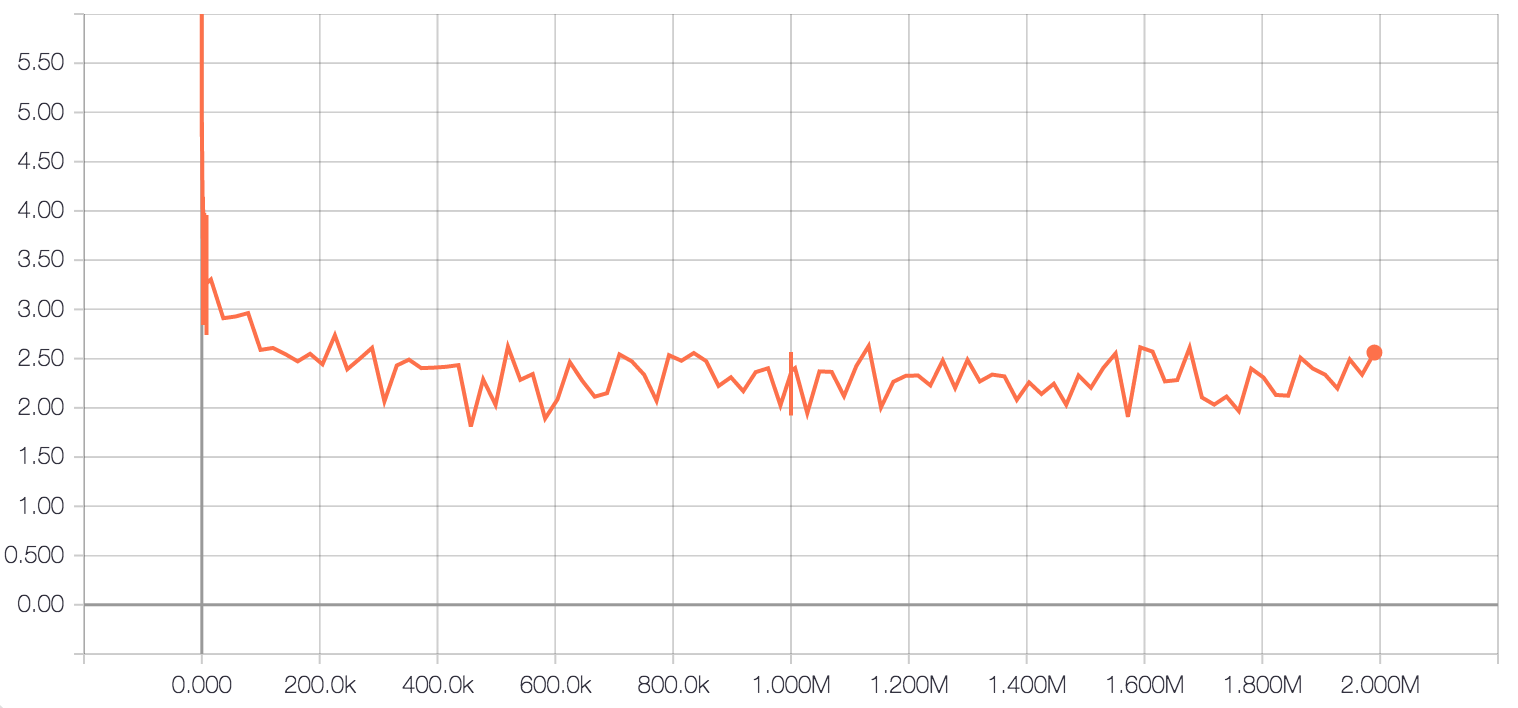
\includegraphics[width=\linewidth]{exp7-1}
  \caption{
    Función de error para el entrenamiento de la LSTM, usando 5 leyendas por personaje,
    un vocabulario reducido y códigos convolucionales generados a partir de una CNN superficial.
    (Fuente: elaboración propia.)
  }
  \label{exp7}
\end{figure}

\begin{figure}[H]
  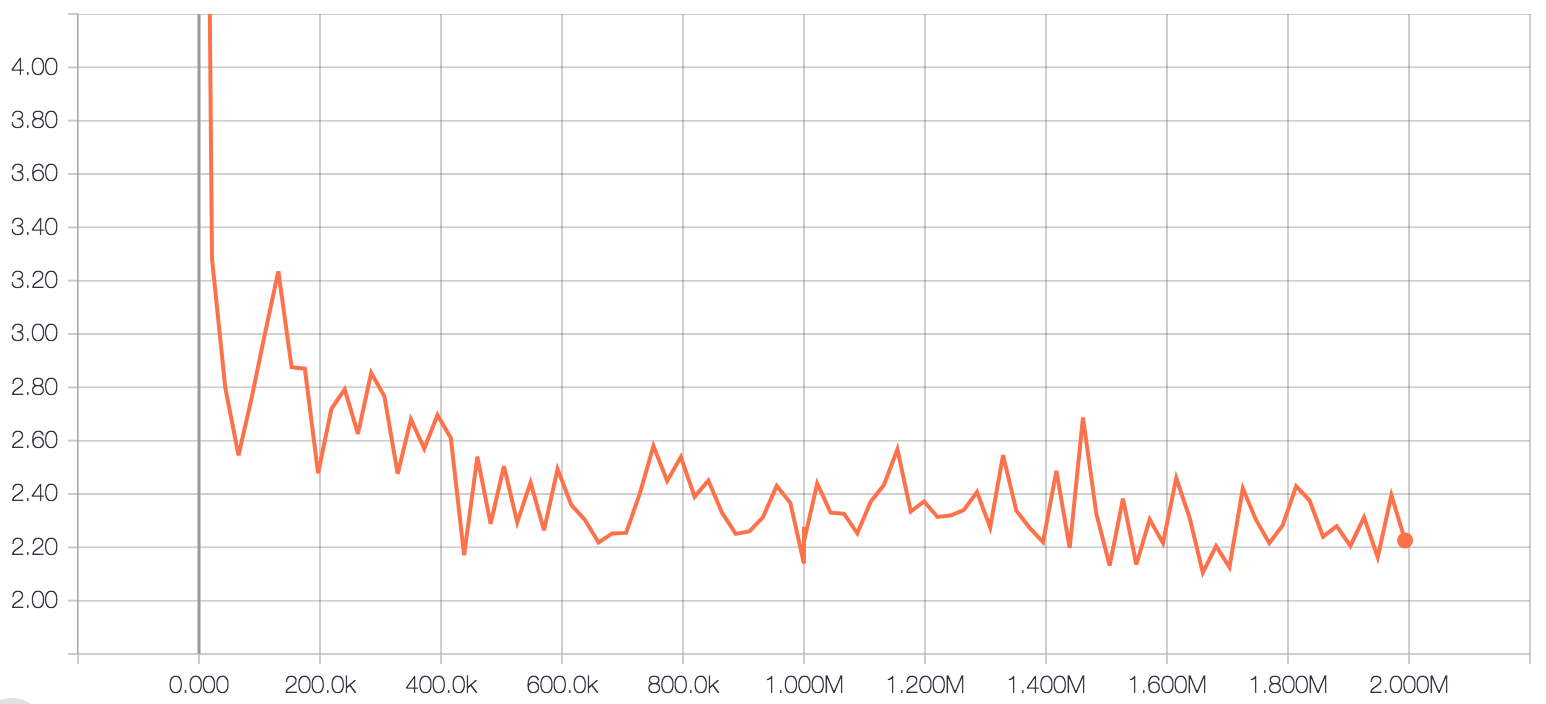
\includegraphics[width=\linewidth]{exp8-1}
  \caption{
    Función de error para el entrenamiento de la LSTM, con códigos convolucionales dados
    por una CNN superficial y 20 leyendas por imagen. Como se observa, existe una ligera
    disminución en el error resultante al final del entrenamiento, con respecto al obtenido
    en experimentos anteriores.
    (Fuente: elaboración propia.)
  }
  \label{exp8}
\end{figure}

Con los mismos datos que para el experimento anterior y con la CNN superficial, se realizó\
el entrenamiento cuyo desempeño se ilustra en la Figura \ref{exp8}. Ahora se aumentó a 20 el\
número de leyendas por imagen. En cuanto a detalles anecdóticos, la Tabla \ref{exp8:anec}\
ilustra una generación de leyendas con un poco de más sentido cuando hay dos palabras\
distintas contiguas. Resumimos los detalles técnicos de todos los experimentos presentados\
en la Tabla \ref{exp-details}.

\begin{table}[H]
  \begin{tabular}{|p{0.5\linewidth}|p{0.2\linewidth}|p{0.3\linewidth}|}
    \hline
    \textbf{tipo de experimento} & \textbf{número de personajes} & \textbf{número de leyendas por personaje}\\
    \hline \hline
    Réplica de entrenamiento de \emph{Inception V3}, como en \cite{DBLP:journals/corr/VinyalsTBE16} & \multicolumn{2}{|c|}{Conjunto de datos \emph{ImageNet}} \\
    \hline
    LSTM a partir de \emph{Inception V3} & 97 & 700, en promedio \\
    \hline
    Afinación de \emph{Inception V3} & \multicolumn{2}{|c|}{3065 memes y 3065 no memes} \\
    \hline
    LSTM a partir de \emph{Inception V3} afinada & 97 & 700, en promedio \\
    \hline
    LSTM a partir de \emph{Inception V3} afinada & 3416 & 5 \\
    \hline
    Entrenamiento de una CNN superficial & \multicolumn{2}{|c|}{3065 memes y 3065 no memes} \\
    \hline
    LSTM a partir de la CNN superficial & 3416 & 5 \\
    \hline
    LSTM a partir de la CNN superficial & 3416 & 20 \\
    \hline
  \end{tabular}
  \caption{
    Resumen de los detalles técnicos presentados en esta sección.
  }
  \label{exp-details}
\end{table}

\section{Evaluación del desempeño de la LSTM} \label{sec:metrics}

\noindent
En el contexto del procesamiento del lenguaje natural, es común preguntarse qué tan \emph{buenos}\
son los enunciados generados con respecto a un lenguaje referencia. En el caso que concierne a esta tesis,\
tratamos con un lenguaje informal, generado a partir de la popularidad que adquieren ciertas frases\
dentro del Internet. Sin embargo, es posible discernir entre un enunciado que hace sentido\
empírico a uno que combina palabras sin patrón alguno.\par
Las métricas propuestas en \cite{DBLP:journals/corr/VinyalsTBE16} sugieren el uso de un corpus\
lingüístico de referencia, con el cual se compare la similitud entre las estructuras gramaticales\
generadas por el modelo con enunciados ``reales''. Por ello, hemos construido un corpus lingüístico
formado por leyendas en el conjunto de \emph{evaluación} para fines de realizar una comparación\
con los resultados emitidos por la LSTM.\par
En particular, analizamos qué tan bien aprende el modelo a predecir la $t$-ésima palabra, a nivel\
probabilístico. Dada la distribución de probabilidad $p$ sobre los enunciados realizados a partir\
de un alfabeto $\Sigma$%
\footnote{
  Es decir, un modelo de lenguaje.
}, definimos la \textbf{perplejidad} $PP(S)$ del modelo como
\begin{equation}
  PP(S) = p(s_1 s_2 \ldots s_n) ^{-\frac{1}{n}}, \label{eq:perplexity0}
\end{equation}
donde $S = s_1, s_2, \ldots, s_n \in S^*$. Desarrollando la Ecuación \ref{eq:perplexity0},\
tenemos que
\begin{align}
  PP(S) &= \sqrt[n]{\frac{1}{p(s_1 s_2 \ldots s_n)}}\\
  &= \sqrt[n]{\prod_{i=0}^n \frac{1}{p(s_{i+1}\ |\ s_1 s_2 \ldots s_i)}} \label{eq:perplexity1}
\end{align}\par
La Ecuación \ref{eq:perplexity1} se obtuvo aplicando la \emph{regla de la cadena} de las probabilidades\
conjuntas a la predicción de cada palabra $s_i$. Lo que este razonamiento nos indica es que\
minimizar la perplejidad de un enunciado $S$ con respecto a un modelo $p$, es lo mismo que\
maximizar la probabilidad de $S$ bajo $p$.\par
Intuitivamente, la \emph{perplejidad} del modelo nos dice el número de posibles candidatos que tiene\
el modelo para la palabra $s_{i+1}$, dadas $s_1, s_2, \ldots, s_i$. Si la \emph{perplejidad} es minimizada,\
entonces el modelo aprende con éxito a descubrir patrones de secuencias de palabras.\par
Queremos comparar los dos \emph{mejores} modelos entrenados, es decir, el mejor de los que\
codifican imágenes con la arquitectura convolucional superficial contra el mejor de los que\
codifican con \emph{Inception V3}. Llamémoslos \verb+Modelo A+ y \verb+Modelo B+, respectivamente.\
Para exponerlos a un conjunto de imágenes ajenas a los datos de entrenamiento, se tomaron 20 ``nuevos\
memes'' (la mayoría, provenientes de sitios web con gran popularidad actual%
\footnote{
  \url{https://www.reddit.com} y \url{https://me.me}.
}), 20 de las imágenes del conjunto de datos de evaluación\
y 20 imágenes nuevas de \emph{ImageNet} (``no memes''). Esta distinción se hizo con el fin de mostrar\
qué tanto aprendió el modelo acerca de los memes y qué tanto generalizó en detalles.\par
Los promedios de las perplejidades arrojadas por cada experimento de\
evaluación se muestran en la Tabla \ref{avgperplexities}. Observamos que la profundidad de la\
CNN del \verb+Modelo B+ brinda un mejor contexto a la LSTM de los\
atributos que constituyen a la imagen de entrada, por lo que se justifica la discrepancia entre las\
perplejidades del \verb+Modelo A+ y del \verb+Modelo B+.\par
Recordemos que la CNN del \verb+Modelo A+ fue entrenada bajo la tarea de distinguir el conjunto de datos\
de memes con un subconjunto de \emph{ImageNet}. Por ello, muchas abstracciones posiblemente identificadas\
por la CNN del \verb+Modelo B+ no logran ser reflejadas en las salidas de la CNN del \verb+Modelo A+.\
Más aún, como la CNN del \verb+Modelo B+ estuvo previamente entrenada con los datos de \emph{ImageNet},\
de los cuales surgen los ``no memes'', es entendible que dicho modelo haya logrado un desempeño similar con\
``no memes'' y memes de evaluación. En contraste, los nuevos memes constituyen una clase de imágenes que no\
fue parte tanto del pre-entrenamiento como de la afinación del \verb+Modelo B+.\par
Los resultados de la evaluación pueden ser consultados de manera\
interactiva en el \textbf{repositorio de código fuente}%
\footnote{
  El repositorio se encuentra en \url{https://github.com/alorozco53/Deep-Meme-Captioner/blob/evaluate/memes/testing.md}.
} de esta tesis.

\begin{table}[H]
  \centering
  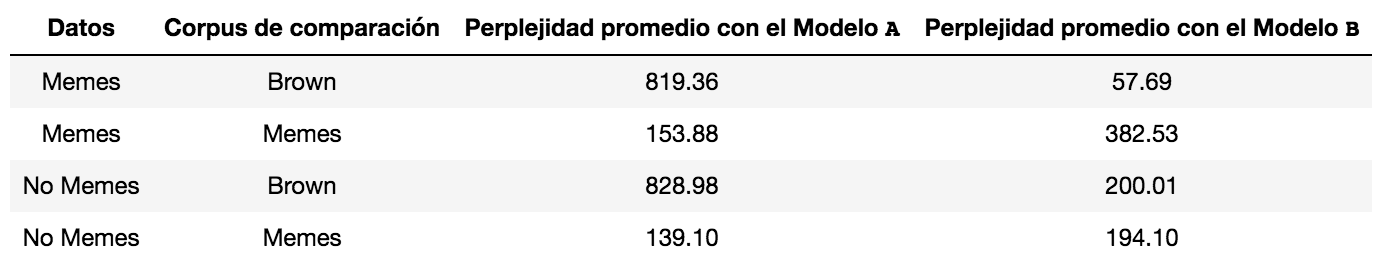
\includegraphics[width=\textwidth]{avgperplexities}
  \caption{
    Promedios de las perplejidades arrojadas al evaluar los dos \emph{mejores} modelos contra el
    \emph{corpus} formado mediante las leyendas de los memes extraídos de Internet.
  }
  \label{avgperplexities}
\end{table}
